\documentclass[a4paper,11pt,openright]{report}
\setlength{\parindent}{0pt} % set noindent for entire file

\usepackage[utf8]{inputenc}
\usepackage[a4paper,top=20mm,bottom=25mm,left=12mm,right=20mm]{geometry}
\usepackage{xcolor,graphicx}
\usepackage{amsmath}
\usepackage{setspace}
\usepackage{sectsty}
\usepackage{etoolbox}
\usepackage{enumitem}
\usepackage{listings}
\usepackage{textcmds}
\usepackage{times}

\graphicspath{ {/home/saran/Analytics/Oct_28/} }

\lstdefinestyle{mystyle}{
	backgroundcolor=\color{white},
	basicstyle=\ttfamily\footnotesize,
	breakatwhitespace=false,
	breaklines=true,
	captionpos=b,
	keepspaces=true,
	showspaces=false,
	showstringspaces=false,
	showtabs=false,
	tabsize=4
}

\lstset{style=mystyle}

\begin{document}
\singlespacing
\pagestyle{plain}

\begin{center}
\textbf{Assignment: Binomial Distribution} \\
Date: 28/10/2020 \hspace{2mm} Name: D.Saravanan
\end{center}

\vspace{10px}

\begin{enumerate}

\item[1.] Find the probability of exactly $15$ successes in $121$ trials with $p = 0.1$

The probability that a random variable $X$ with binomial distribution $B(n,p)$ is equal to
the value $k$, where $k = 0, 1,...n$, is given by

\begin{equation*}
P(X = k) = \binom nk p^{k} (1-p)^{n-k} = \frac{n!}{k! (n-k)!} p^{k} (1-p)^{n-k}
\end{equation*}

\begin{equation*}
\begin{split}
P(X = 15) & = \binom{121}{15} (0.1)^{15} (1-0.1)^{106} \\
& = \frac{121!}{15! (121-15)!} (0.1)^{15} (0.9)^{106} \\
& = 0.07622452
\end{split}
\end{equation*}

Script: 
\lstinputlisting[language=R]{program1.R}

Output:
\lstinputlisting{output1.txt}

%figure_1
\begin{figure}[ht!]
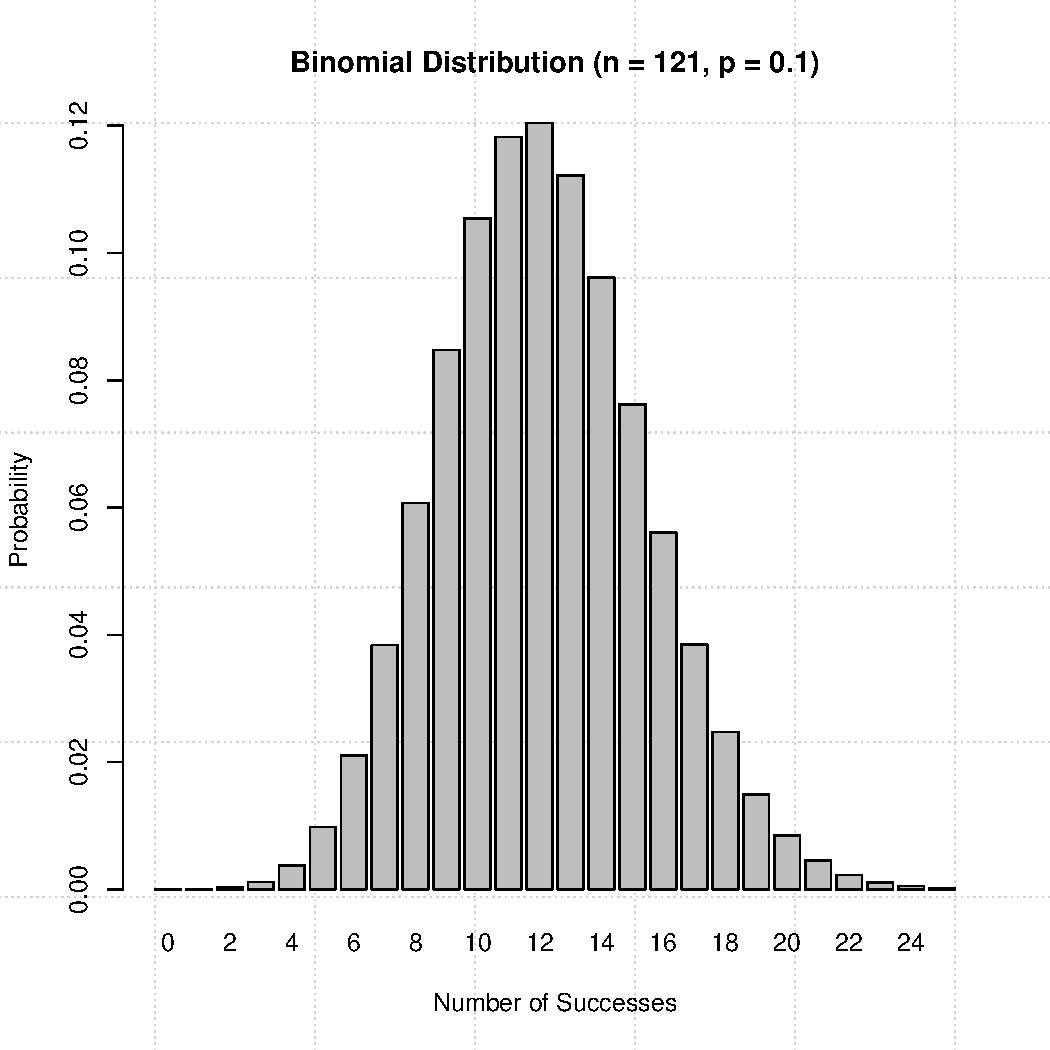
\includegraphics[width=16cm,height=8cm,keepaspectratio]{plot1.pdf}
\centering
\end{figure}

\pagebreak

\item[2.] Find the probability that in $30$ tosses of a fair coin the head comes up with
less than $24$ times.

\begin{equation*}
\begin{split}
P(X < 24) & = P(X \leq 23) \\
		  & = 1 - (1 - P(X \leq 23)) \\
		  & = 1 - P(X \geq 24) \\
		  & = 1 - \bigg( P(X = 24) + P(X = 25) + P(X = 26) \\
		  &\quad + P(X = 27) + P(X = 28) + P(X = 29) + P(X = 30) \bigg) \\
		  & = 1 - \Bigg( \binom{30}{24} (0.5)^{24} (1-0.5)^{6} + \binom{30}{25} (0.5)^{25} (1-0.5)^{5} + \binom{30}{26} (0.5)^{26} (1-0.5)^{4} \\
		  &\quad + \binom{30}{27} (0.5)^{27} (1-0.5)^{3} + \binom{30}{28} (0.5)^{28} (1-0.5)^{2} + \binom{30}{29} (0.5)^{29} (1-0.5) + \binom{30}{30} (0.5)^{30} \Bigg) \\
		  & = 1 - \Bigg( \frac{30!}{24! (30-24)!} (0.5)^{24} (0.5)^{6} +  \frac{30!}{25! (30-25)!} (0.5)^{25} (0.5)^{5} +  \frac{30!}{26! (30-26)!} (0.5)^{26} (0.9)^{4} \\
		  &\quad +  \frac{30!}{27! (30-27)!} (0.5)^{27} (0.5)^{3} +  \frac{30!}{28! (30-28)!} (0.5)^{28} (0.5)^{2} +  \frac{30!}{29! (30-29)!} (0.5)^{29} (0.5) \\
		  &\quad +  \frac{30!}{30! (30-30)!} (0.5)^{30} \Bigg) \\
		  & = 1 - \Big( 0.0005529961 + 0.0001327191 + 0.0000255229 \\
		  &\quad + 0.0000037812 + 0.0000004051 + 0.0000000279 + 0.0000000009 \Big) \\
		  & = 0.9992845
\end{split}
\end{equation*}

Script:
\lstinputlisting[language=R]{program2.R}

Output:
\lstinputlisting{output2.txt}

%figure_2
\begin{figure}[ht!]
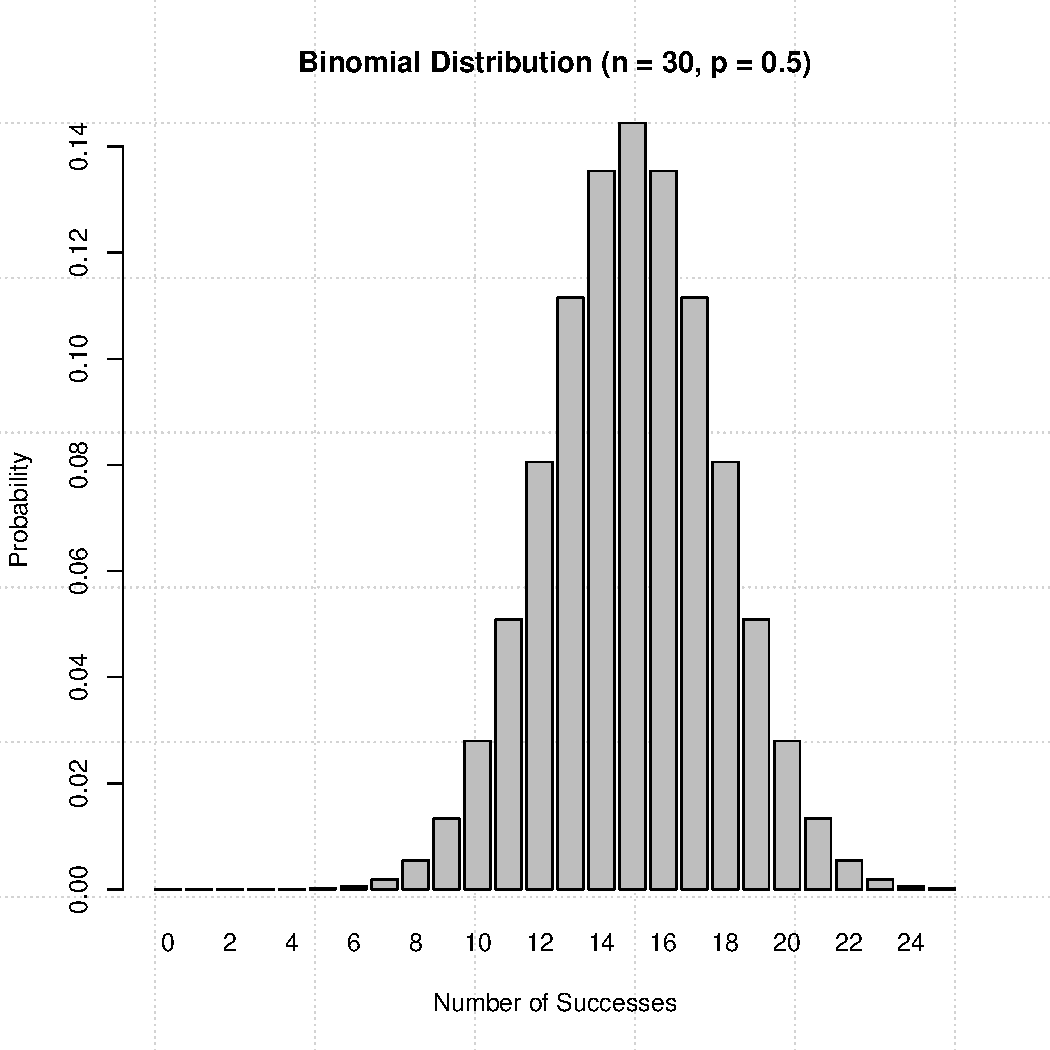
\includegraphics[width=16cm,height=8cm,keepaspectratio]{plot2.pdf}
\centering
\end{figure}

\pagebreak

\item[3.] Find the probability that in $75$ tosses of a fair coin the tail comes up between
$28$ and $32$ times.

\begin{equation*}
\begin{split}
P(28 \leq X \leq 32) & = P(X = 28) + P(X = 29) + P(X = 30) + P(X = 31) + P(X = 32) \\
					 & = \binom{75}{28} (0.5)^{28} (1-0.5)^{47} + \binom{75}{29} (0.5)^{29} (1-0.5)^{46} + \binom{75}{30} (0.5)^{30} (1-0.5)^{45} \\
					 &\quad + \binom{75}{31} (0.5)^{31} (1-0.5)^{44} + \binom{75}{32} (0.5)^{32} (1-0.5)^{43} \\
					 & = \frac{75!}{28! (75-28)!} (0.5)^{28} (0.5)^{47} + \frac{75!}{29! (75-29)!} (0.5)^{29} (0.5)^{46} + \frac{75!}{30! (75-30)!} (0.5)^{30} (0.5)^{45} \\
					 &\quad + \frac{75!}{31! (75-31)!} (0.5)^{31} (0.5)^{44} + \frac{75!}{32! (75-32)!} (0.5)^{32} (0.5)^{43} \\
					 & = 0.00832825 + 0.01349751 + 0.02069618 + 0.03004284 + 0.0413089 \\
					 & = 0.1138737
\end{split}
\end{equation*}

Script:
\lstinputlisting[language=R]{program3.R}

Output:
\lstinputlisting{output3.txt}

%figure_3
\begin{figure}[ht!]
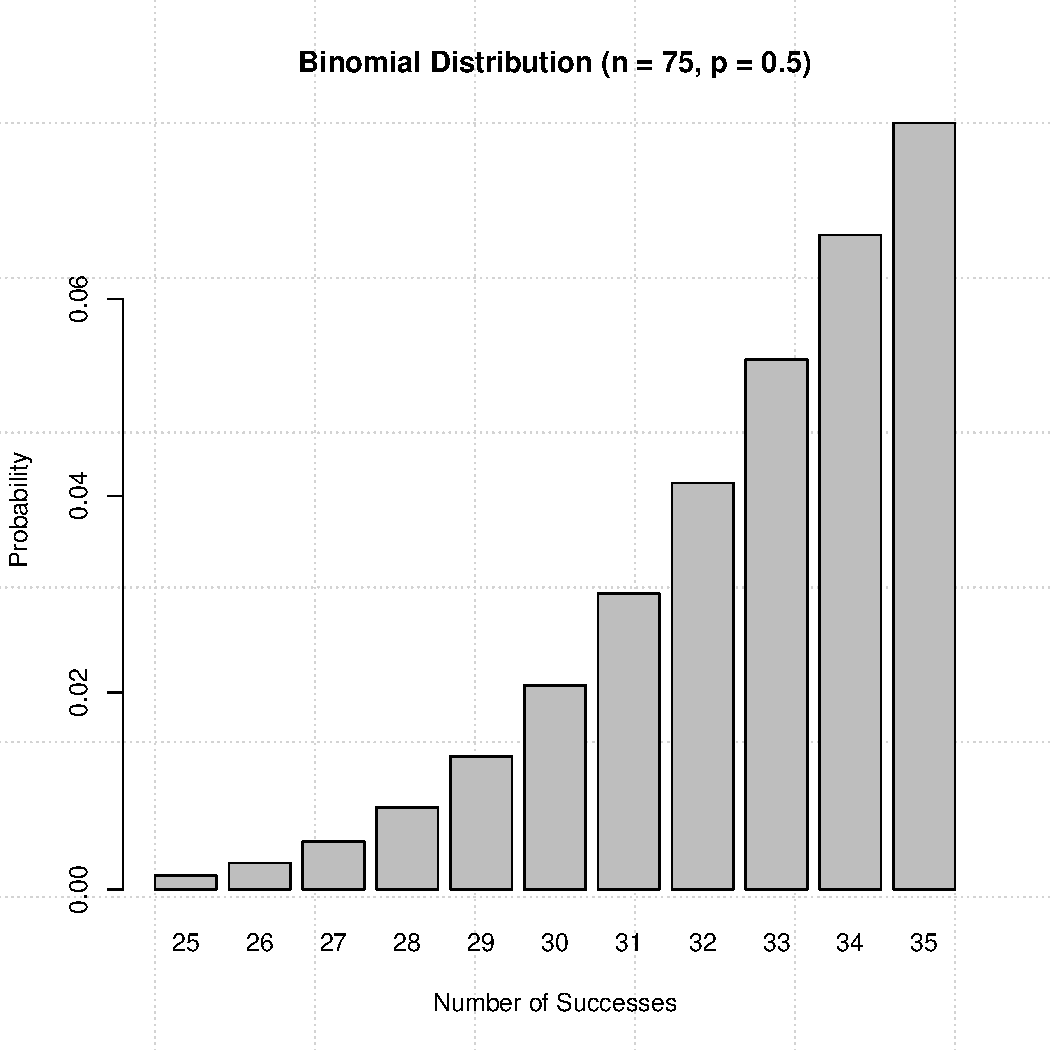
\includegraphics[width=16cm,height=8cm,keepaspectratio]{plot3.pdf}
\centering
\end{figure}

\item[4.] How many heads will have a probability of $0.80$ will come out when a coin is
tossed $25$ times.

Script:
\lstinputlisting[language=R]{program4.R}

Output:
\lstinputlisting{output4.txt}

%figure_4
\begin{figure}[ht!]
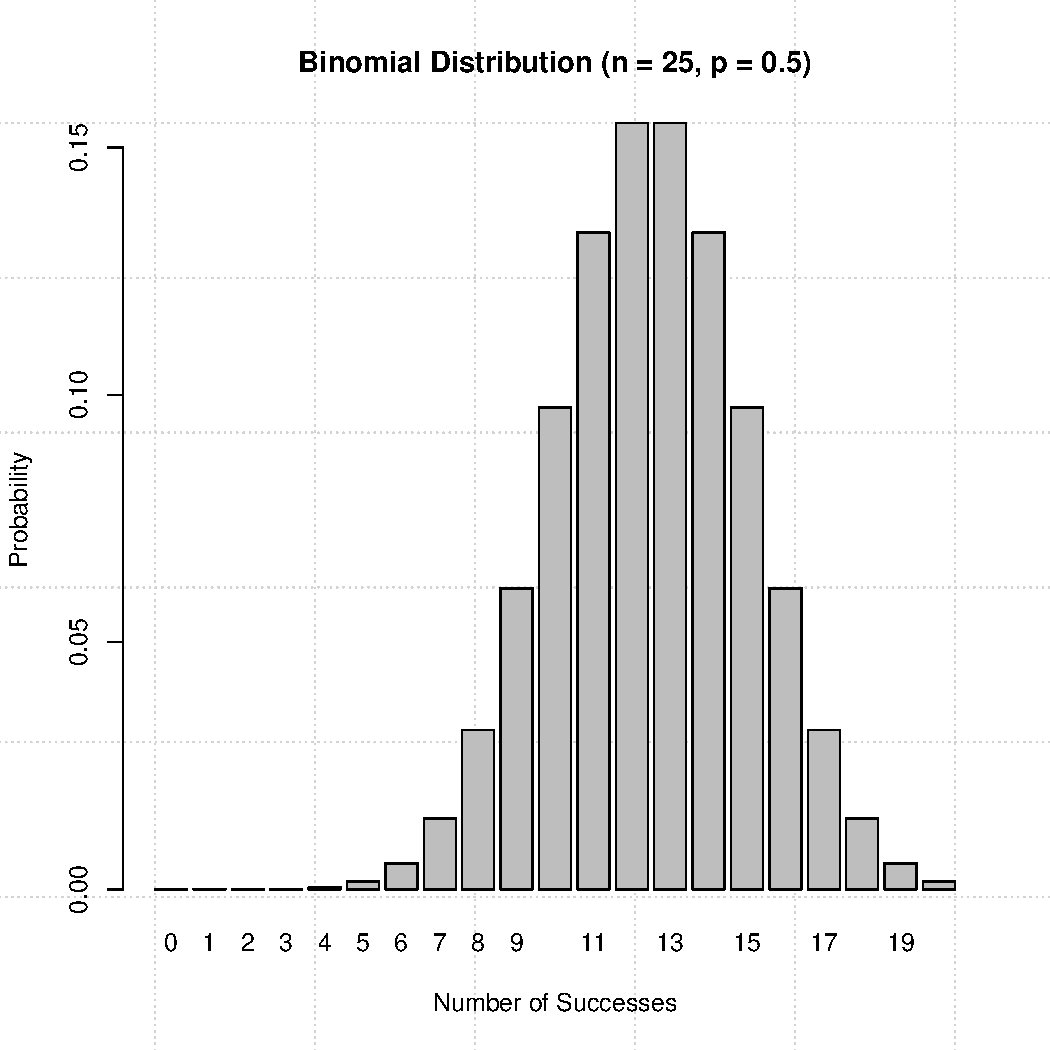
\includegraphics[width=16cm,height=8cm,keepaspectratio]{plot4.pdf}
\centering
\end{figure}

\end{enumerate}
\end{document}
